\documentclass[pdflatex,compress]{beamer}

%\usetheme[dark,framenumber,totalframenumber]{ElektroITK}
\usetheme[darktitle,framenumber,totalframenumber]{ElektroITK}

\renewcommand{\figurename}{Gambar} \setbeamertemplate{caption}[numbered]

\usepackage{graphicx}
\usepackage{multicol}

\title{FORENSIKA SUARA}
\subtitle{Konsep Dasar Sinyal dan Sistem Audio}

\author{Tim Dosen Pengampu}

\begin{document}

\maketitle

\section{Pendahuluan}

\begin{frame}
	\frametitle{Pendahuluan}
	\begin{itemize}
		\item Ilmu akustik dan audio engineering merupakan dasar dari audio forensik.
		\item Bukti audio forensik meliputi audio recording. \item Representasi dari bunyi yang dideteksi di udara oleh mikrofon, dikonversi menjadi tegangan, dan kemudian disimpan dalam suatu media.
		\item Rekaman audio bisa berupa analog maupun digital.
		\item Studi tentang akustik melibatkan prinsip fisika dari propagasi bunyi di udara.
	\end{itemize}
\end{frame}

\begin{frame}
	\frametitle{Pendahuluan}
	\begin{itemize}
		\item Untuk memahami dan menginterpretasikan rekaman forensik, perlu memahami konsep akustik sehingga bunyi yang dideteksi di dalam rekaman dapat dianalisis dan dikaitkan dengan karakteristik pemantulan (reflection), penyerapan (absorption), difraksi (diffraction), dan dengung (reverberation) dari bunyi.
	\end{itemize}
\end{frame}

\section{Bunyi}

\begin{frame}
	\frametitle{Bunyi}
	\begin{itemize}
		\item Bunyi di udara merupakan hasil dari getaran.
		\item Permukaan yang bergetar menyebabkan partikel-partikel bergerak maju mundur dalam jarak pendek.
		\item Permukaan bergerak ke depan $\rightarrow$ partikel udara di dekat permukaan didorong (compressed), permukaan bergerak mundur $\rightarrow$ partikel udara di dekat permukaan ditarik (expanded/rarified).
		\item Partikel udara yang mengalami compressed-expanded tadi akan melakukan hal yang sama terhadap partikel udara di dekatnya, dan seterusnya.
		\item Menghasilkan gelombang yang menjauhi permukaan yang bergetar.
	\end{itemize}
\end{frame}

\begin{frame}
	\frametitle{Gerakan partikel udara}
	\begin{figure}
		\centering
		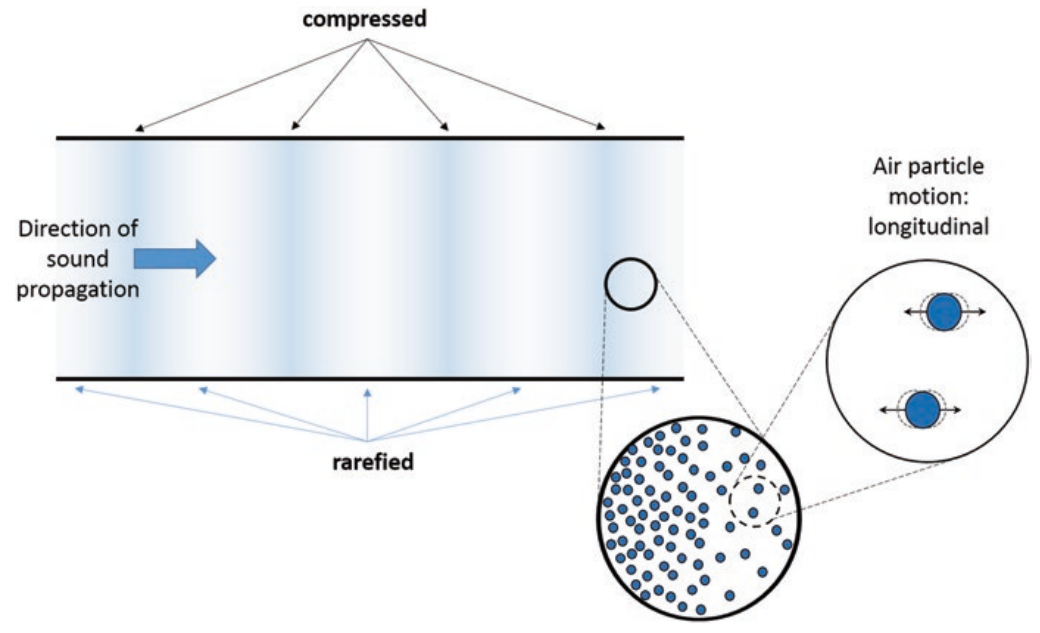
\includegraphics[width=0.7\linewidth]{img/img001}
		\caption[]{Gerakan partikel udara di dalam gelombang bunyi: longitudinal (maju dan mundur) sejajar dengan arah propagasi.}
		\label{fig:img001}
	\end{figure}
\end{frame}

\begin{frame}
	\frametitle{Tekanan akustik}
	\begin{itemize}
		\item Gelombang bunyi adalah gelombang longitudinal.
		\item Karena gerakan longitudinal sulit untuk digambarkan, maka penggambarannya berdasarkan tekanan akustik terhadap waktu.
		\item Tekanan akustik sangat kecil jika dibandingkan dengan tekanan atmosfir normal.
		\item Tekanan di atas permukaan laut $ \approx 1 \times 10^5 $ Pa.
		\item Suara terkecil yang dapat didengar memiliki tekanan sebesar $ 2 \times 10^{-5} $ Pa.
		\item Suara yang sangat keras (konser atau mesin di industri) $\approx$ 1 Pa.
	\end{itemize}
\end{frame}

\section{Tingkat Tekanan Bunyi}

\begin{frame}
	\frametitle{Tingkat Tekanan Bunyi}
	\begin{itemize}
		\item Sound pressure level (SPL) / tingkat tekanan bunyi.
		\item Tekanan akustik yang dapat didengar berada di rentang $ 2 \times 10^{-5} $ hingga 1 Pa.
		\item Rentang yang dapat didengar diubah ke dalam satuan logaritmik agar bunyi yang paling senyap berada pada level zero dan yang paling keras berada di dalam 2 atau 3 angka saja.
		\[ B = \log_{10}\frac{(\text{daya}_1)}{(\text{daya}_0)} \] atau 
		\[ B = \log_{10}\frac{(\text{intensitas}_1)}{(\text{intensitas}_0)} \]
		\item B adalah bel, daya dalam Watt dan intensitas dalam W/m$ ^2 $
	\end{itemize}
\end{frame}

\begin{frame}
	\frametitle{Tingkat Tekanan Bunyi}
	\begin{itemize}
		\item Agar dapat menggunakan definisi bel di atas untuk bunyi, perlu dilakukan konversi dari tekanan akustik (pascal) ke intensitas akustik (W/m$ ^2 $).
		\item Hubungan antara gelombang bunyi adalah intensitas akustik proporsional dengan kuadrat dari tekanan akustik, sehingga
		\[ B = \log_{10}\frac{(\text{tekanan}_1^2)}{(\text{tekanan}_0^2)} = 2\log_{10}\frac{(\text{tekanan}_1)}{(\text{tekanan}_0)} \]
		\item decibel [dB] = presisi 1/10 dari bel.
		\[ \text{decibel}[dB] = 20 \log_{10} \frac{tekanan_1}{tekanan_0}  \]
	\end{itemize}
\end{frame}

\begin{frame}
	\frametitle{Tingkat Tekanan Bunyi}
	\begin{itemize}
		\item SPL dalam decibel $\rightarrow \text{tekanan}_0 = 20~ \mu\text{Pa}$ dan $ \text{tekanan}_1 $ = tekanan efektif atau RMS yang diukur di mikrofon.
		\item Dipilih 20 $\mu$Pa karena batas dari pendengaran manusia.
		\item Jika ada sinyal akustik dengan tekanan efektif sebesar 20 $\mu$Pa, maka SPL nya adalah 0 dB.
		\item Gelombang bunyi yang berpropagasi di udara memiliki kecepatan bunyi sebesar 343 m/s dalam suhu ruang 20$^\circ$C.
	\end{itemize}
\end{frame}

\section{Panjang Gelombang, Frekuensi dan Spektrum}
\begin{frame}
	\frametitle{Panjang Gelombang dan Frekuensi}
	\begin{itemize}
		\item Jika sumber suara berosilasi, bunyi akan memiliki siklus tekanan tinggi dan rendah.
		\item Waktu yang dibutuhkan dalam satu kali osilasi disebut periode getaran.
		\item Selama waktu yang dibutuhkan dalam 1 kali osilasi, tekanan bunyi akan berpropagasi di udara sejauh jarak tertentu. Jarak ini disebut panjang gelombang.
		\item Osilasi bunyi diekspresikan dalam laju osilasi, yaitu berapa banyak siklus osilasi dalam 1 detik.
		\item Laju osilasi ini yang disebut dengan frekuensi.
	\end{itemize}
\end{frame}

\begin{frame}
	\frametitle{Panjang Gelombang dan Frekuensi}
	\begin{itemize}
		\item Jika osilasinya sedikit (frekuensinya rendah), periode dari tiap siklus akan berdurasi tinggi, sehingga gelombang akan berpropagasi lebih jauh dalam satu siklus.
		\item Frekuensi lebih rendah $\rightarrow$ panjang gelombang lebih panjang.
		\item Begitu juga sebaliknya.
		\item Hubungan antara frekuensi $ f $ dan panjang gelombang $ \lambda $ adalah $ c = f\lambda $, dimana $ c $ adalah kecepatan bunyi (m/s).
	\end{itemize}
\end{frame}

\begin{frame}
	\frametitle{Panjang Gelombang dan Frekuensi}
	\begin{figure}
		\centering
		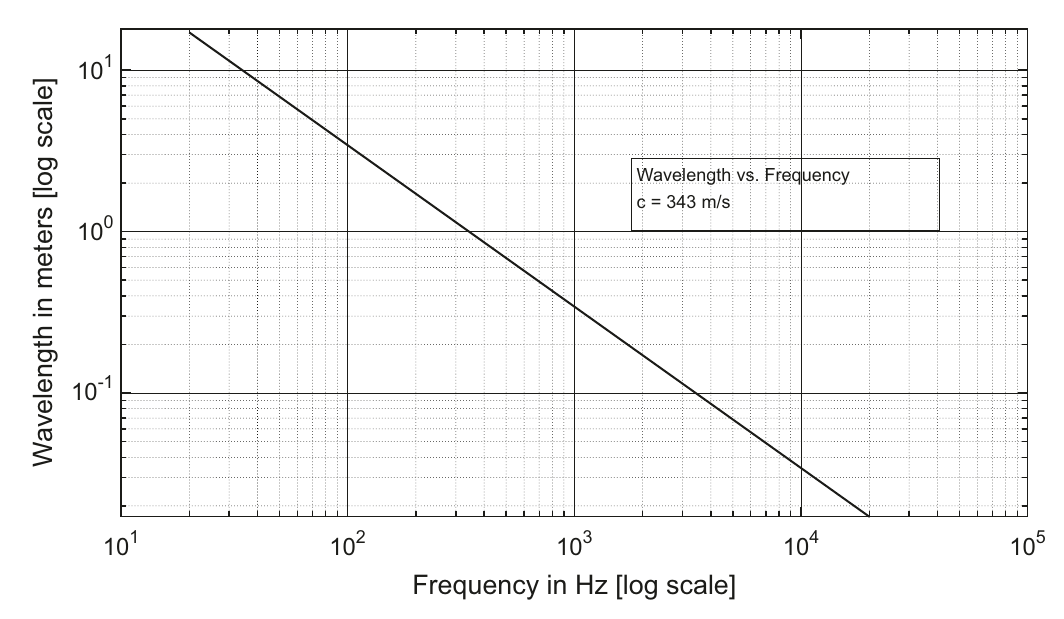
\includegraphics[width=0.9\linewidth]{img/img002}
		\caption{Perkalian antara frekuensi terhadap panjang gelombang adalah kecepatan bunyi.}
		\label{fig:img002}
	\end{figure}
\end{frame}

\begin{frame}
	\frametitle{Sinewave}
	\begin{itemize}
		\item Jenis paling sederhana dari bunyi yang memiliki energi pada frekuensi tunggal adalah pure tone.
		\item Bentuk gelombang (waveform) dari bunyi frekuensi tunggal ini seperti pada Gambar \ref{fig:img003}.
		\item Disebut juga sinewave atau sinusoidal.
		\item Sumbu y dapat berupa tekanan, tegangan, atau perpindahan (displacement) dan sumbu x adalah waktu.
		\item Gambar \ref{fig:img003} memiliki T = 1 md dan frekuensi = 1/T = 1 kHz.
		\item Untuk sinewave dengan interval yang lebih lama ditunjukkan oleh Gambar \ref{fig:img004}.
	\end{itemize}
\end{frame}

\begin{frame}
	\frametitle{Sinewave}
	\begin{figure}
		\centering
		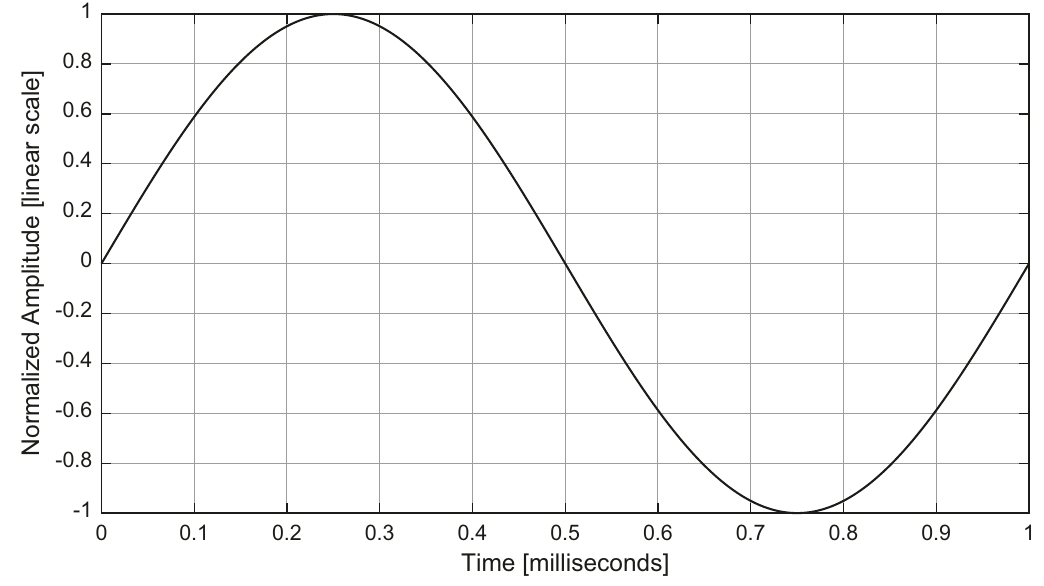
\includegraphics[width=0.7\linewidth]{img/img003}
		\caption{Sinewave 1 kHz}
		\label{fig:img003}
	\end{figure}
\end{frame}

\begin{frame}
	\frametitle{Sinewave}
	\begin{figure}
		\centering
		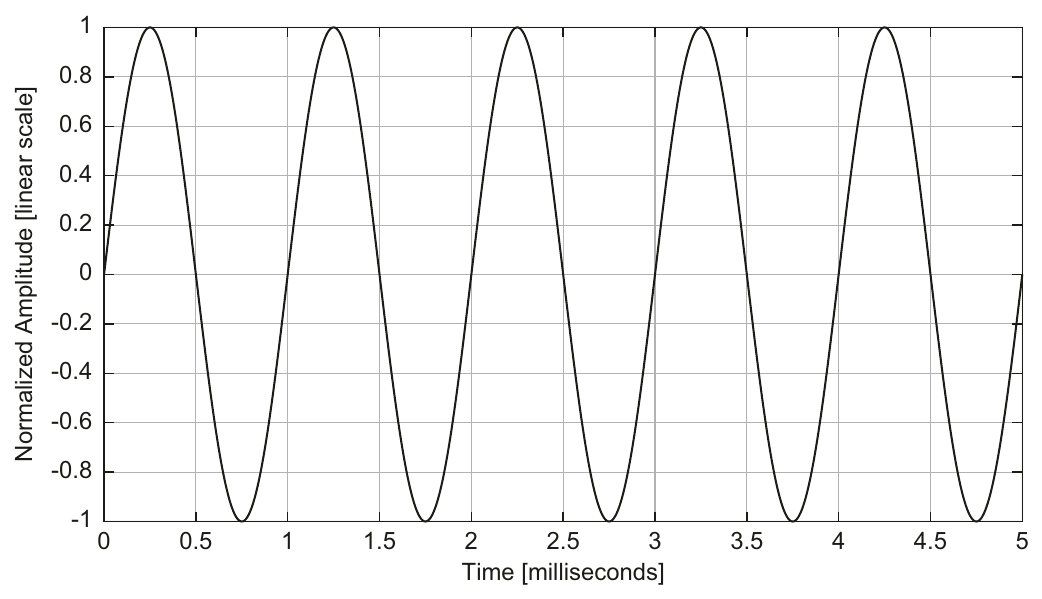
\includegraphics[width=0.7\linewidth]{img/img004}
		\caption{Sinewave 1 kHz dengan 5 siklus}
		\label{fig:img004}
	\end{figure}
\end{frame}

\begin{frame}
	\frametitle{Spektrum}
	\begin{itemize}
		\item Waveform yang periodik memiliki spektrum yang harmonik.
		\item Artinya energi hanya ada pada frekuensi yang merupakan kelipatan bilangan bulat dari frekuensi dasar/fundamental frequency ($ f_0 $).
		\item Gambar \ref{fig:img005} merupakan spektrum dari sinewave 1kHz puretone.
	\end{itemize}
\end{frame}

\begin{frame}
	\frametitle{Spektrum}
	\begin{figure}
		\centering
		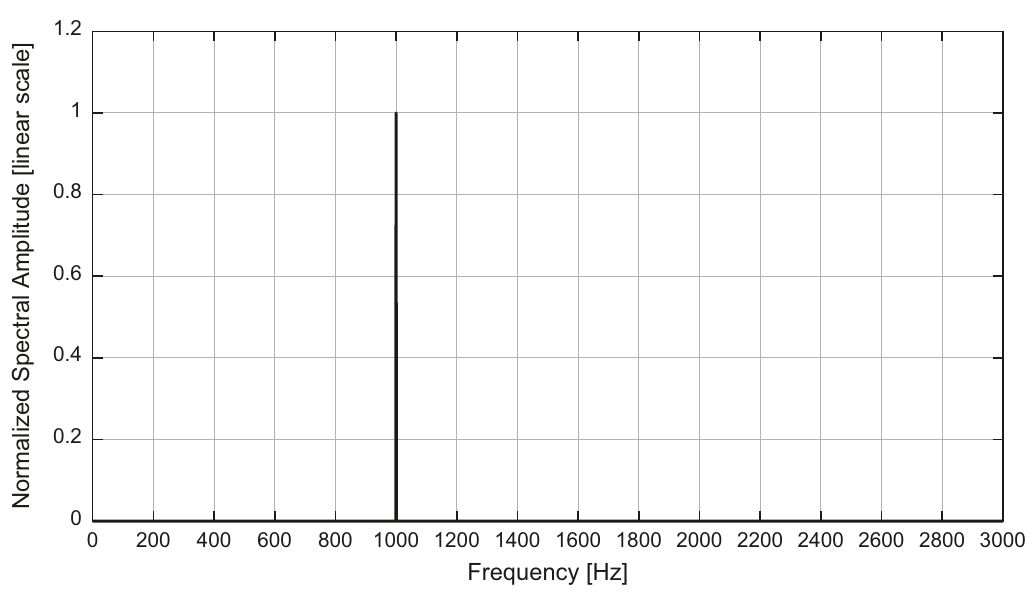
\includegraphics[width=0.7\linewidth]{img/img005}
		\caption{Magnitudo spektrum frekuensi 1 kHz puretone}
		\label{fig:img005}
	\end{figure}
\end{frame}

\begin{frame}
	\frametitle{Waveform dan Spektrum}
	\begin{itemize}
		\item Gambar \ref{fig:img006} adalah waveform periodik dan Gambar \ref{fig:img007} adalah magnitude spektrumnya.
		\item Gambar \ref{fig:img007} dapat diperoleh dengan menggunakan deret Fourier.
		\item Selain itu, transformasi Fourier dapat digunakan untuk menentukan spektrum dari waveform nonperiodik seperti yang ditunjukkan oleh Gambar \ref{fig:img008} dan Gambar \ref{fig:img009}.
		\item Nanti akan dijelaskan cara memperoleh waveform dan spektrum menggunakan Google Colab.
	\end{itemize}
\end{frame}

\begin{frame}
	\frametitle{Waveform dan Spektrum}
	\begin{multicols}{2}
		\begin{figure}
			\centering
			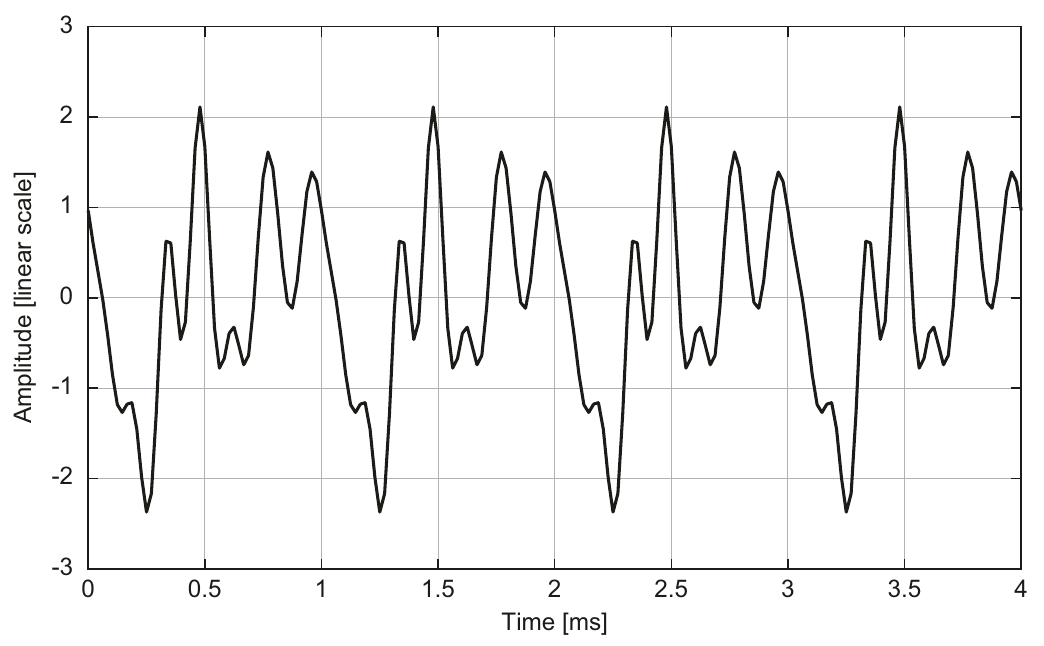
\includegraphics[width=\linewidth]{img/img006}
			\caption{Contoh waveform periodik dengan frekuensi dasar 1 kHz}
			\label{fig:img006}
		\end{figure}
		\columnbreak
		\begin{figure}
			\centering
			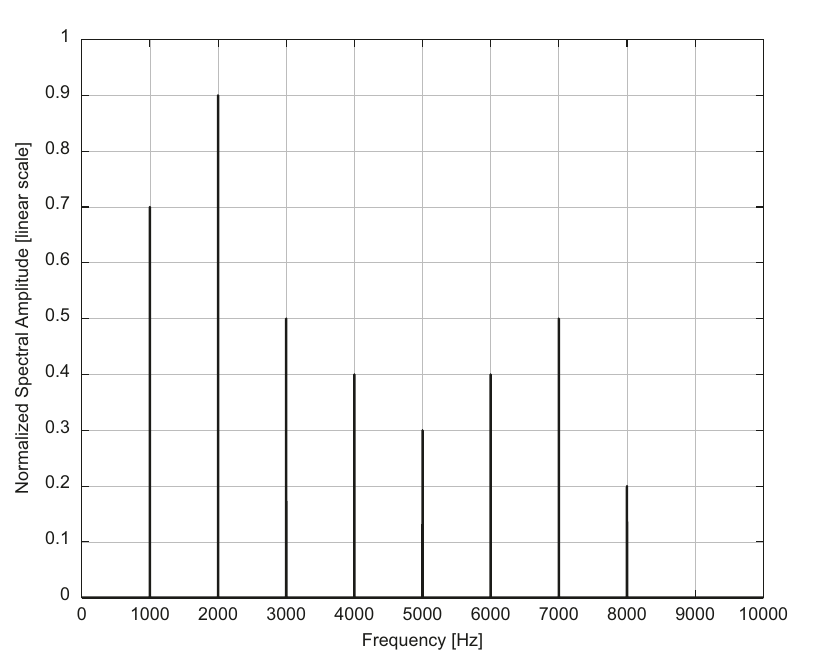
\includegraphics[width=\linewidth]{img/img007}
			\caption{Spektrum frekuensi dari waveform periodik dengan frekuensi dasar 1 kHz}
			\label{fig:img007}
		\end{figure}
	\end{multicols}
\end{frame}

\begin{frame}
	\frametitle{Spektrum dari Waveform Nonperiodik}
	\begin{multicols}{2}
		\begin{figure}
			\centering
			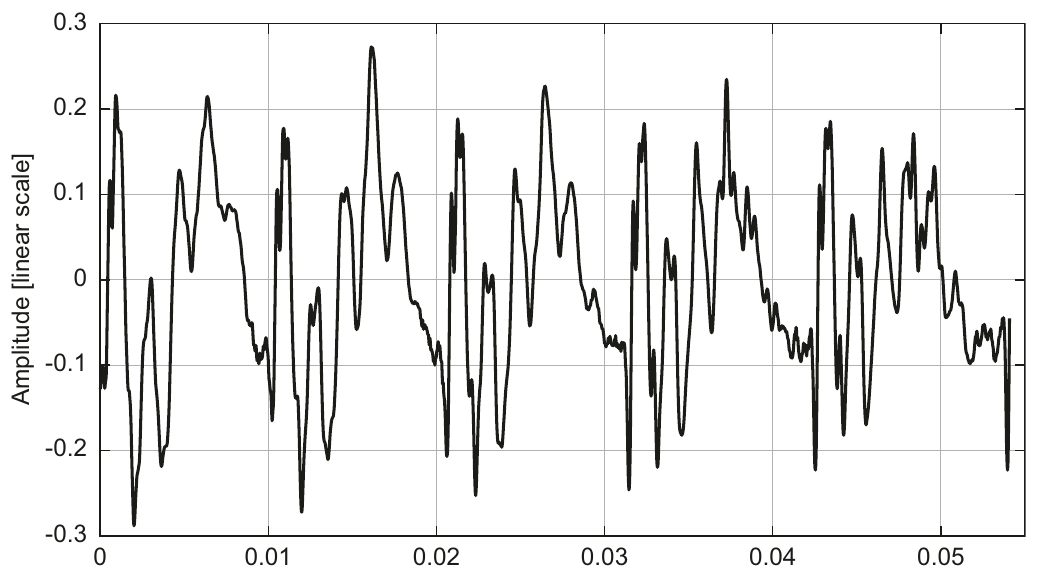
\includegraphics[width=\linewidth]{img/img008}
			\caption{Waveform nonperiodik dari sinyal suara}
			\label{fig:img008}
		\end{figure}
		\columnbreak
		\begin{figure}
			\centering
			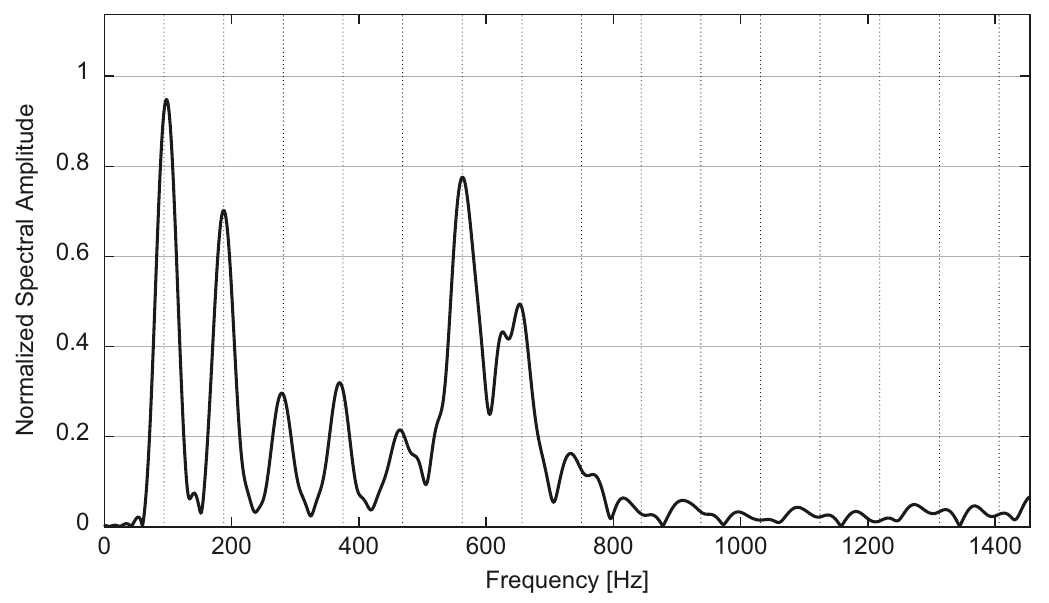
\includegraphics[width=\linewidth]{img/img009}
			\caption{Spektrum frekuensi dari waveform nonperiodik}
			\label{fig:img009}
		\end{figure}
	\end{multicols}
\end{frame}

\begin{frame}
	\frametitle{Octave}
	\begin{itemize}
		\item Octave: frekuensi dasar dari suatu sinyal adalah dua kalinya dari frekuensi dasar sinyal lain.
		\item Satu octave di atas puretone 200 Hz adalah 400 Hz.
		\item Dua octave di atas puretone 200 Hz adalah 800 Hz.
	\end{itemize}
\end{frame}

\section{Propagasi Gelombang}
\begin{frame}
	\frametitle{Propagasi Gelombang}
	\begin{itemize}
		\item Gelombang bunyi di udara berpropagasi menjauhi sumber bunyi ke segala arah/ spherical wave.
		\item Saat berpropagasi, energi bunyi dari sumber akan terdistribusi ke permukaan spherical tersebut.
		\item Semakin jauh dari sumber bunyi, daya bunyi akan berkurang.
		\item Jika tidak ada pantulan bunyi, luas permukaan spherical sebanding terhadap radius kuadrat ($ 4\pi r^2 $).
		\item Sehingga intensitas bunyi (watt/satuan luas) menurun sebesar 1/($ r^2 $).
		\item Intensitas bunyi sebanding dengan kuadrat tekanan bunyi, sehingga tekanan bunyi menurus sebesar 1/r.
	\end{itemize}
\end{frame}

\begin{frame}
	\frametitle{Penurunan SPL}
	\begin{itemize}
		\item Faktor 1/r untuk penurunan tekanan bunyi dengan meningkatnya jarak menghasilkan penurunan 6 db SPL setiap penggandaan jarak.
		
		\[ 20 \log_{10}((1/r) \times \frac{P}{P_{ref}}) = 20 \log_{10}(\frac{P}{P_{ref}}) - 20 \log_{10}(r) \]
		
		Jika r berubah dari 1 ke 2 (penggandaan jarak), maka
		
		\[ -20 \log_{10}(2) = -6.02 \text{ dB}\]
		\item Namun pada kenyataannya, propagasi gelombang sphrical membentur suatu permukaan, sehingga teori tadi tidak berlaku karenan adanya superposisi dari pantulan bunyinya.
	\end{itemize}
\end{frame}

\begin{frame}
	\frametitle{Kecepatan Bunyi}
	\begin{itemize}
		\item Kecepatan bunyi di udara bervariasi terhadap temperatur udara (Gambar \ref{fig:img010}).
		\item Bunyi akan berpropagasi lebih cepat di udara yang hangat dari lebih lambat di udara dingin.
		\item Bunyi dengan frekuensi tertentu $\rightarrow$ panjang gelombang lebih panjang di udara hangat daripada di udara dingin.
		\item Bagaimana jika kondisi temperatur udaranya bergradient (Semakin tinggi semakin hangat suhunya) ?
	\end{itemize}
\end{frame}

\begin{frame}
	\frametitle{Kecepatan Bunyi}
	\begin{figure}
		\centering
		
\includegraphics[width=\linewidth]{img/img010}
		\caption{Kecepatan bunyi di udara merupakan fungsi dari temperatur udara.}
		\label{fig:img010}
	\end{figure}
\end{frame}

\begin{frame}
	\frametitle{Refraksi Akibat Beda Temperatur}
	\begin{multicols}{2}
		\begin{figure}
			\centering
			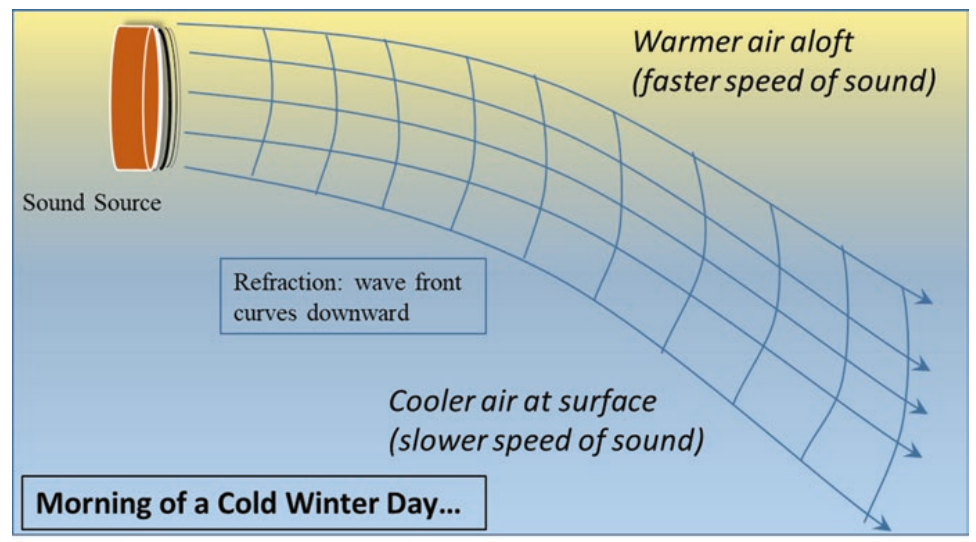
\includegraphics[width=\linewidth]{img/img011a}
			\caption{Efek refraksi akibat perbedaan temperatur udara, udara dingin di permukaan.}
			\label{fig:img011a}
		\end{figure}
		\columnbreak
		\begin{figure}
			\centering
			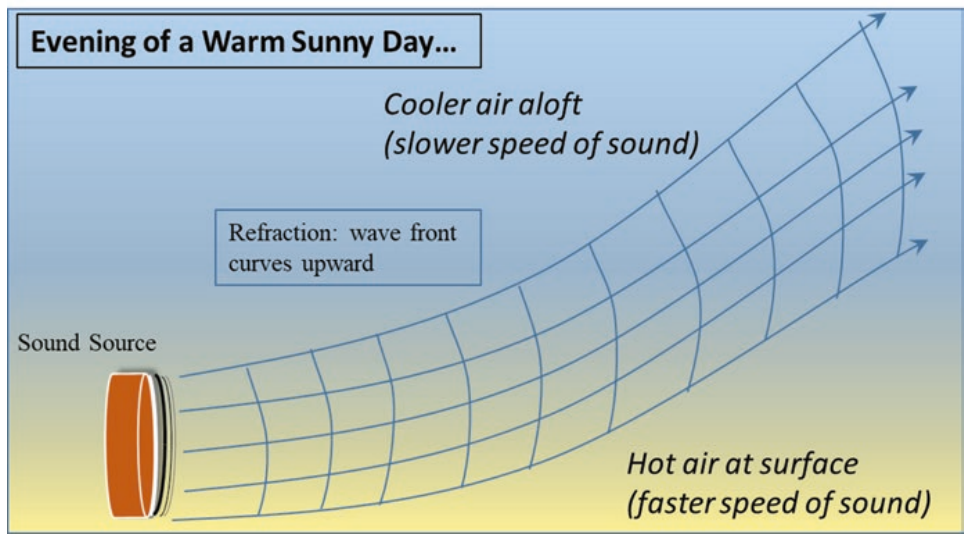
\includegraphics[width=\linewidth]{img/img011b}
			\caption{efek refraksi akibat perbedaan temperatur udara, udara hangat di permukaan.}
			\label{fig:img011b}
		\end{figure}
	\end{multicols}
\end{frame}

\begin{frame}
	\frametitle{Bunyi Langsung dan Pantulan}
	\begin{itemize}
		\item Mikrofon mendeteksi tekanan akustik sesaat, yang terdiri dari
		\begin{enumerate}
			\item gelombang bunyi yang perpropagasi langsung melalui udara dari sumber bunyi ke mikrofon,
			\item gelombang bunyi yang sampai ke mikrofon setelah dipantulkan oleh lantai, dinding, dan permukaan lainnya,
			\item bunyi dengung/reverberant yang datang setelah beberapa pantulan.
		\end{enumerate}
		\item Sehingga audio rekaman berisikan informasi sumber bunyi dan karakteristik akustik dari lingkungan sekitarnya saat rekaman tersebut dibuat.
		\item Jika ada bunyi latar, maka akan dideteksi oleh mikrofon juga.
	\end{itemize}
\end{frame}

\begin{frame}
	\frametitle{Bunyi Langsung dan Pantulan}
	\begin{figure}
		\centering
		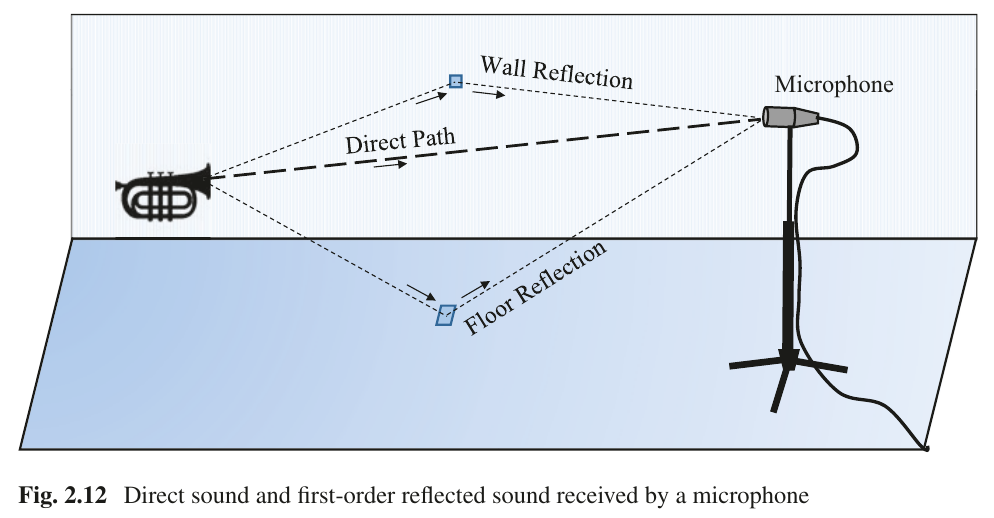
\includegraphics[width=\linewidth]{img/img012}
		\caption{Bunyi langsung dan bunyi pantulan orde pertama yang diterima oleh mikrofon.}
		\label{fig:img012}
	\end{figure}
\end{frame}

\begin{frame}
	\frametitle{Bunyi Pantulan}
	\begin{itemize}
		\item Pantulan yang paling mudah dideteksi/ didengar/ dirasakan adalah ketika permukaan bidang pantul jaraknya jauh dari sumber dan mikrofon.
		\item Semakin jauh jarak pantulannya maka bunyi pantulnya akan sampai di mikrofon jauh setelah bunyi langsung, sehingga menghasilkan echo/ gema.
		\item Jika sumber dan mikrofon jaraknya dekat dengan bidang pantul, delay antara bunyi langsung dan pantulan akan sangat kecil dan tak terasa oleh pendengar tapi tetap dapat dideteksi di dalam audio rekaman.
	\end{itemize}
\end{frame}

\begin{frame}
	\frametitle{Bunyi Pantulan}
	\begin{itemize}
		\item Jika cepat rambat bunyi diketahui, selisih waktu kedatangan dari bunyi langsung dan bunyi pantulan dapat dihitung.
		\item Hasil kali antara cepat rambat bunyi dan selisih waktu kedatangan ini menghasilkan selisih jarak antara bunyi langsung dan bunyi pantul.
		\item Informasi ini yang nantinya dapat digunakan untuk menetukan geometri kejadian di TKP/ crime scene.
	\end{itemize}
\end{frame}

\begin{frame}
	\frametitle{Bunyi Diffuse}
	\begin{itemize}
		\item Bunyi yang berpropagasi di dalam ruangan mengakibatkan mikrofon menerima superposisi dari bunyi langsung dan bunyi pantul/dengung.
		\item Di dalam ruangan yang besar dengan sumber bunyi yang kontinyu, energi bunyi dengung di dalam ruangan ini akan terdistribusi secara uniform.
		\item Bunyi dengung akan datang dari segala arah, sehingga medan bunyi ini disebut difuse.
	\end{itemize}
\end{frame}

\begin{frame}
	\frametitle{Bunyi Dengung/ Reverberant}
	\begin{itemize}
		\item Jika mikrofon berada di dekat sumber bunyi, audio rekaman biasanya akan didominasi oleh bunyi langsung dibandingkan dengan bunyi dengung.
		\item Jika mikrofon bergerak menjauhi sumber bunyi, level dari dengung latar di dalam ruangan akan sama tetapi amplitudo tekanan bunyi langsung akan berkurang sebesar 1/r efek dari propagasi spherical.
		\item Efeknya adalah keseimbangan antara bunyi langsung dan dengung ruangan dalam rekaman akan berubah dari yang didominasi oleh bunyi langsung menjadi didominasi oleh dengung seiring dengan bertambahnya jarak antara sumber bunyi dan mikrofon.
	\end{itemize}
\end{frame}

\begin{frame}
	\frametitle{Bunyi Dengung/ Reverberant}
	\begin{figure}
		\centering
		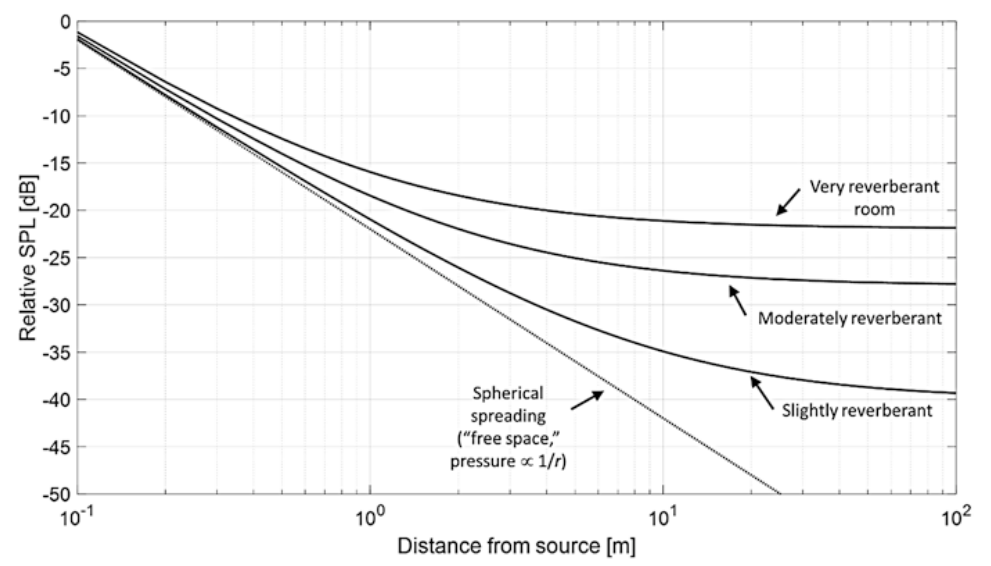
\includegraphics[width=0.9\linewidth]{img/img013}
		\caption{SPL dari mikrofon yang bergerak menjauhi sumber bunyi di ruangan berdengung}
		\label{fig:img013}
	\end{figure}
\end{frame}

\section{Keterarahan Mikrofon}

\begin{frame}
	\frametitle{Keterarahan Mikrofon}
	\begin{itemize}
		\item Karakteristik keterarahan dari mikrofon juga berperan penting dalam merekam sinyal.
		\item Mikrofon secara umum akan merespon tekanan bunyi di diafragma.
		\item Designer mikrofon akan merekayasa mikrofon tersebut lebih merespon bunyi dari arah tertentu saja atau meminimalkan pengaruh/respon dari arah lainnya dengan tujuan mengurangi tingkat tekanan bunyi yang tidak diinginkan.
	\end{itemize}
\end{frame}

\begin{frame}
	\frametitle{Keterarahan Mikrofon}
	\begin{itemize}
		\item Ada 3 jenis karakteristik keterarahan dari mikrofon:
		\begin{enumerate}
			\item omnidirectional,
			\item bidirectional,
			\item unidirectional.
		\end{enumerate}
		\item Pola keterarahan ditunjukkan dengan polar diagram yang menggambarkan jumlah relatif bunyi yang diambil sebagai fungsi dari arah yang ditunjuk oleh mikrofon tersebut.
	\end{itemize}
\end{frame}

\begin{frame}
	\frametitle{Mikrofon omnidirectional}
	\begin{figure}
		\centering
		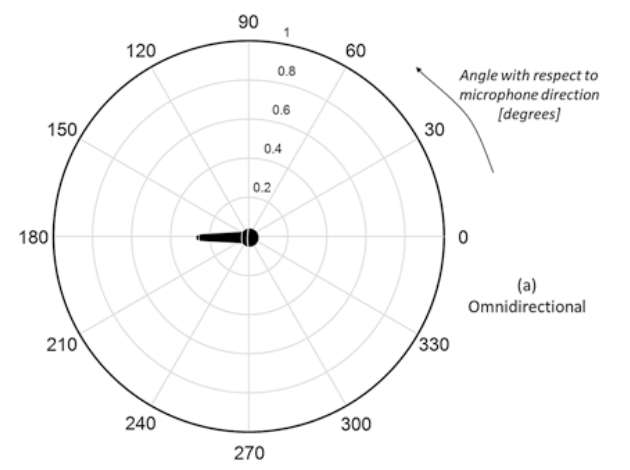
\includegraphics[width=0.6\linewidth]{img/img014a}
		\caption{Diagram pola keterarahan dari mikrofon omnidirectional}
	\end{figure}
\end{frame}

\begin{frame}
	\frametitle{Mikrofon bidirectional}
	\begin{figure}
		\centering
		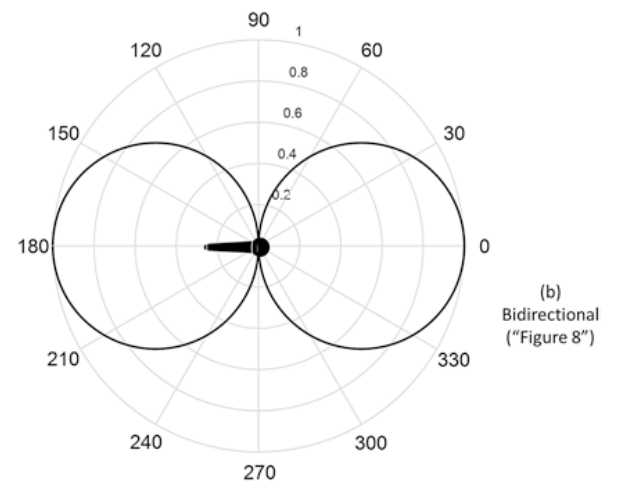
\includegraphics[width=0.6\linewidth]{img/img014b}
		\caption{Diagram pola keterarahan dari mikrofon bidirectional}
	\end{figure}
\end{frame}

\begin{frame}
	\frametitle{Mikrofon unidirectional}
	\begin{figure}
		\centering
		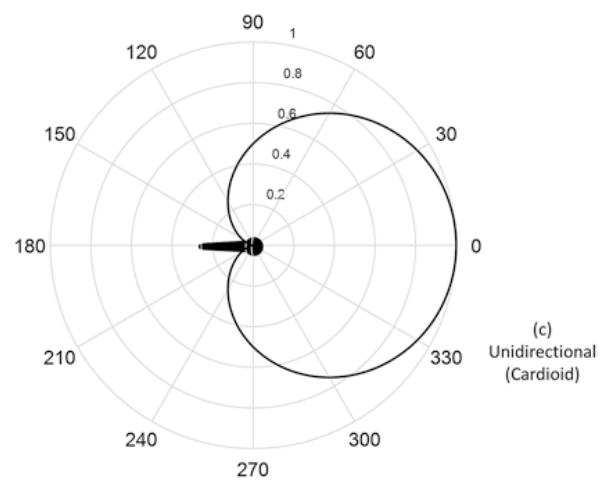
\includegraphics[width=0.6\linewidth]{img/img014c}
		\caption{Diagram pola keterarahan dari mikrofon unidirectional}
	\end{figure}
\end{frame}

\section{Karakteristik Pendengaran Manusia}

\begin{frame}
	\frametitle{Karakteristik Pendengaran Manusia}
	\begin{itemize}
		\item Dalam audio forensik, terkadang melibatkan beberapa pertanyaan terkait kemampuan pendengaran manusia.
		\item Apakah seseorang dapat mendengarkan bunyi dalam kondisi tertentu?
		\item Misalkan, apakah bunyi alarm masih terdengar ada jarak tertentu, atau pada saat ada bunyi lain yang menggangu.
		\item Permasalahan di atas memerlukan pemahaman terkait kekuatan dan kelemahan dari sistem pendengaran manusia.
	\end{itemize}
\end{frame}

\subsection{Anatomi dan Fisiologi Telinga}

\begin{frame}
	\frametitle{Telinga}
	\begin{itemize}
		\item Telinga: organ sensory yang mentransduksi energi bunyi ke dalam neural code yang kemudian diproses oleh otak.
		\item Anatomi dasar dari telinga dibagi menjadi 3 bagian: telinga bagian luar, telinga bagian tengah, dan telinga bagian dalam.
		\begin{center}
			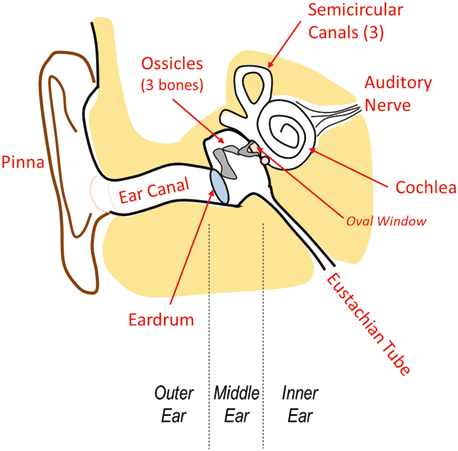
\includegraphics[width=0.5\linewidth]{img/img015}
		\end{center}
	\end{itemize}
\end{frame}

\begin{frame}
	\frametitle{Telinga Bagian Luar}
	\begin{center}
		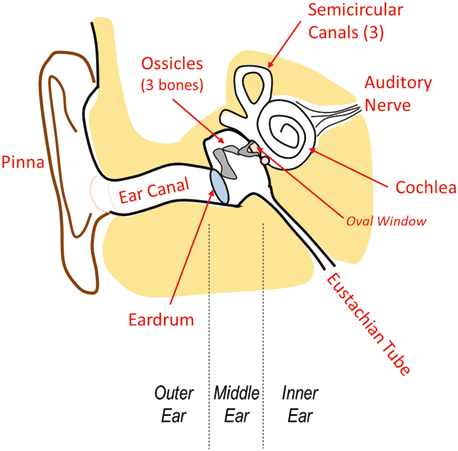
\includegraphics[height=0.9\textheight]{img/img015}
	\end{center}
\end{frame}

\begin{frame}
	\frametitle{Telinga Bagian Luar}
	\begin{itemize}
		\item Banyak mamalia yang memiliki movable pinna, tapi tidak untuk manusia.
		\item Ear canal: 0.8 cm - 2.5 cm.
		\item Tekanan udara di dalam kanal sama dengan tekanan udara ambient-nya.
		\item Bagian paling dalam dari ear canal terdapat tympanic membrane/ eardrum/ gendang telinga yang kedap udara dan kedap air tapi masih mungkin terjadinya akustik koupling langsung dari bunyi luar.
	\end{itemize}
\end{frame}

\begin{frame}
	\frametitle{Telinga Bagian Luar}
	\begin{multicols}{2}
		\begin{center}
			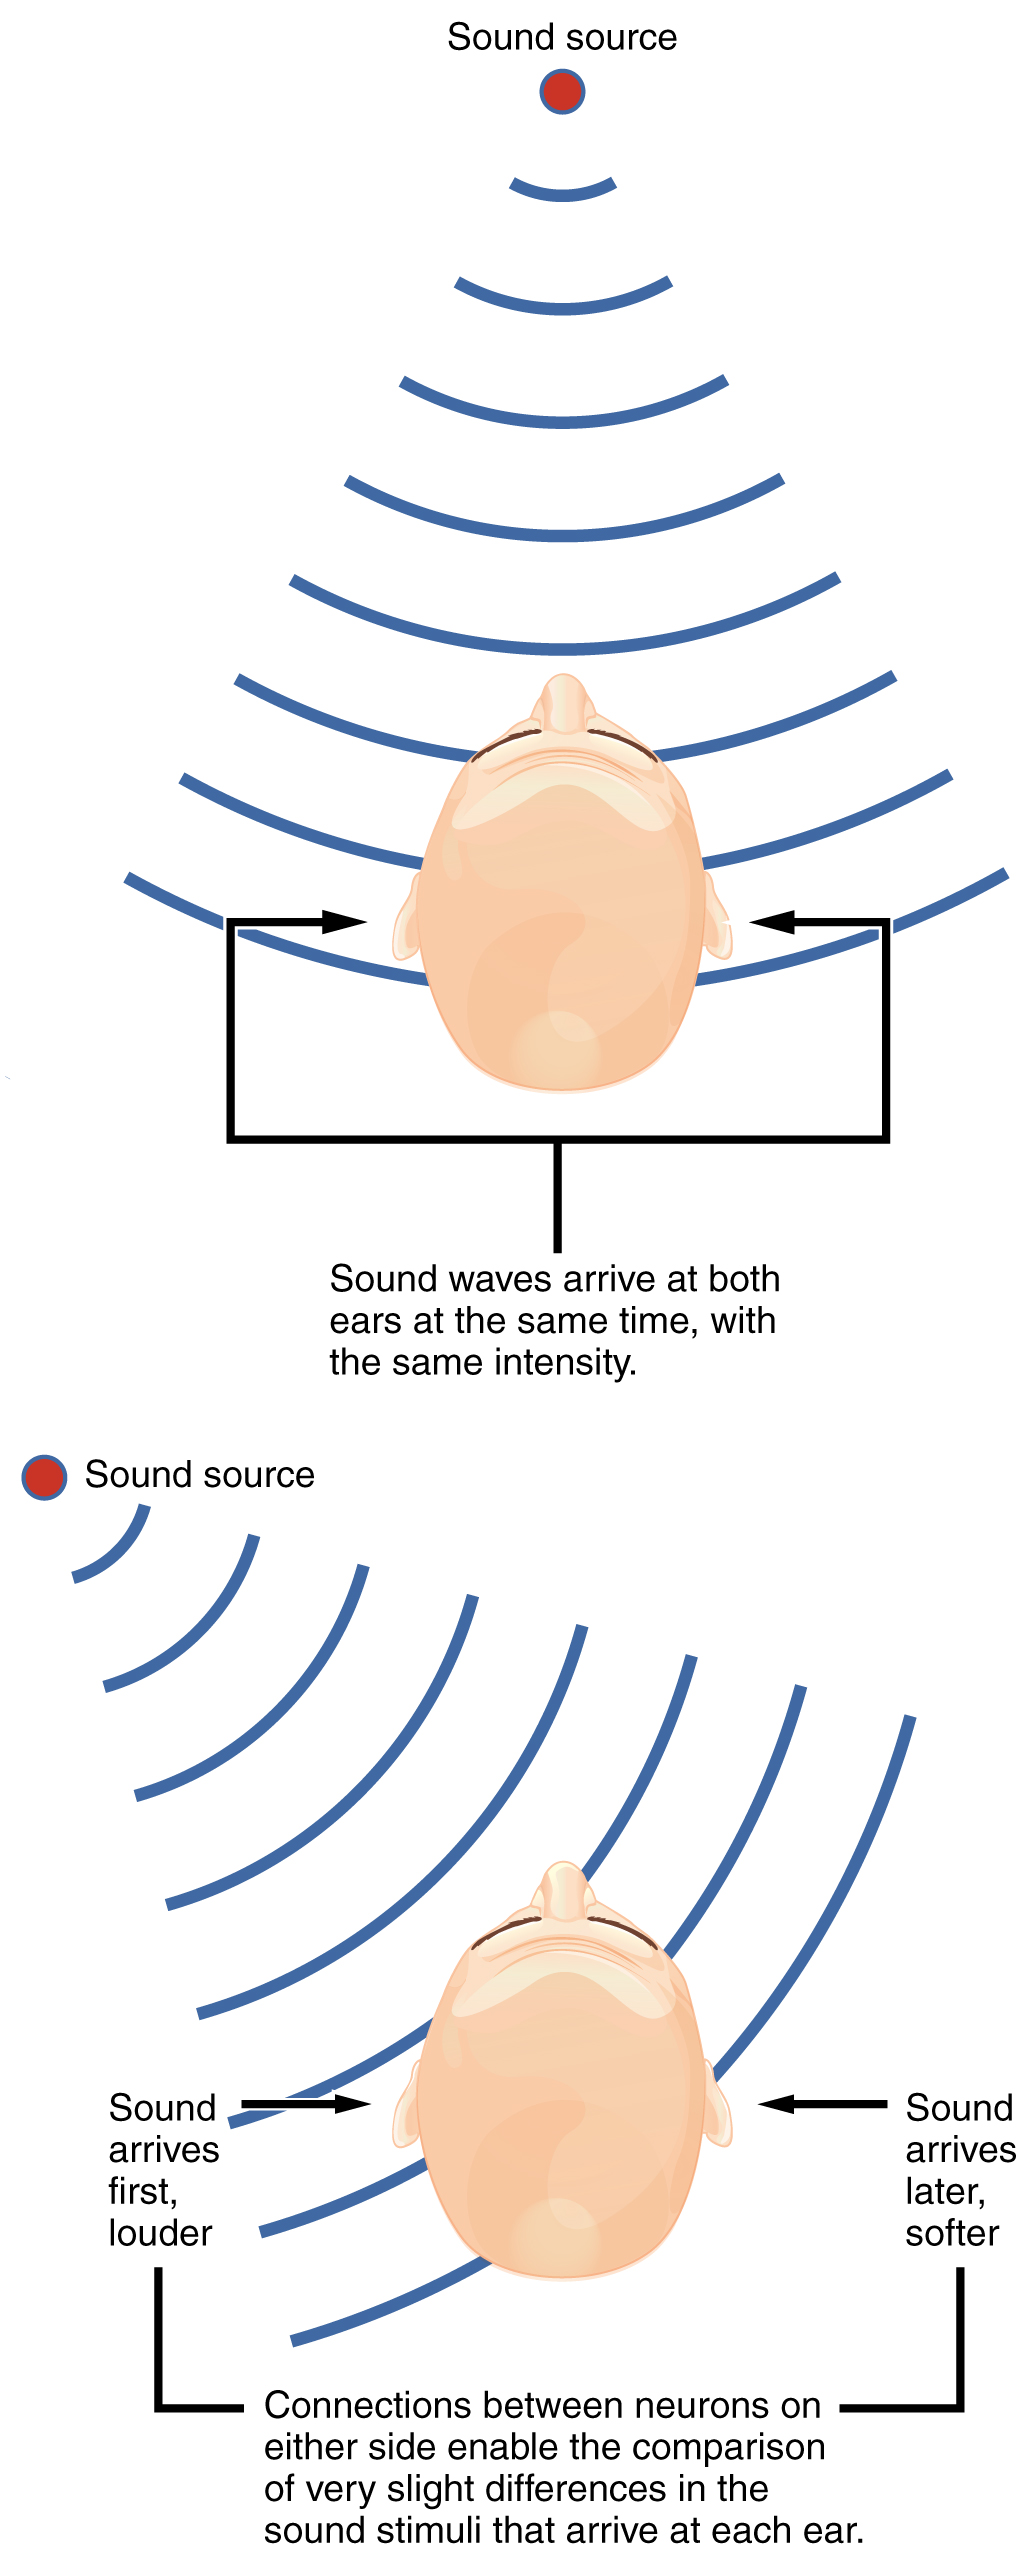
\includegraphics[height=0.9\textheight]{img/img016}
		\end{center}
		\columnbreak
		\begin{itemize}
			\item Bentuk dan struktur dari telinga bagian luar serta posisi dari telinga terhadap kepala dan tubuh bagian atas, menyebabkan difraksi akustik yang bergantung pada azimuth \& elevasi dari sumber bunyi dan panjang gelombang dari bunyi.
			\item Menyebabkan manusia dapat mendeteksi arah sumber bunyi $\rightarrow$ binaural hearing
		\end{itemize}
	\end{multicols}
\end{frame}

\begin{frame}
	\frametitle{Telinga Bagian Tengah}
	\begin{center}
		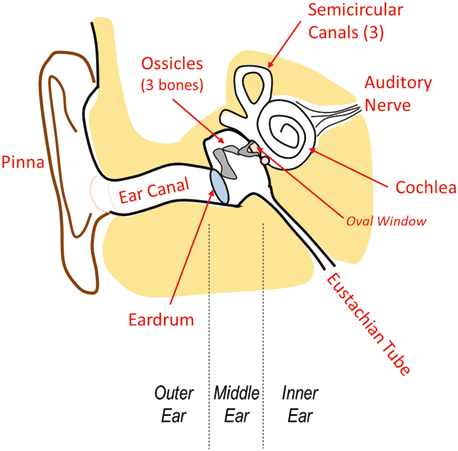
\includegraphics[height=0.9\textheight]{img/img015}
	\end{center}
\end{frame}

\begin{frame}
	\frametitle{Telinga Bagian Tengah}
	\begin{itemize}
		\item Telinga bagian tengah: di antara eardrum dan telinga bagian dalam.
		\item Terdapat 3 ossicles (tiny bones) \& tympanic cavity.
		\item Ossicles = malleus/ hammer terhadap permukaan bagian dalam dari eardrum.
		\item Incus/anvil dan stapes/stirrup terhubung ke oval windows dari teliga bagian dalam.
		\item Eustachian tube: kanal antara middle ear cavity dan bagian belakang nashopharynx.
		\item Perbedaan tekanan $\rightarrow$ udara mengalir di dalam eustachian tube $\rightarrow$ sensasi yang kita rasakan saat naik pesawat/gunung.
	\end{itemize}
\end{frame}

\begin{frame}
	\frametitle{Telinga Bagian Dalam}
	\begin{itemize}
		\item Telinga bagian dalam terdapat:
		\begin{enumerate}
			\item Cochlea
			\item Tiga semicircular canal
			\item Struktur-struktur yang membentuk vestibular organ keseimbangan.
		\end{enumerate}
		\item Tiga semicircular canal sensitif terhadap kecepatan angular dalam ruang 3 dimensi.
		\item Dua semicircular canal yang paling kecil sensitif terhadap percepatan linear yang berkaitan dengan gravitasi.
		\item Cochlea merupakan organ neosensory yang paling penting dalam sistem pendengaran.
		\item Cochlea sensitif terhadap getaran yang disebabkan oleh bunyi.
	\end{itemize}
\end{frame}

\begin{frame}
	\frametitle{Proses Pendengaran}
	\begin{center}
		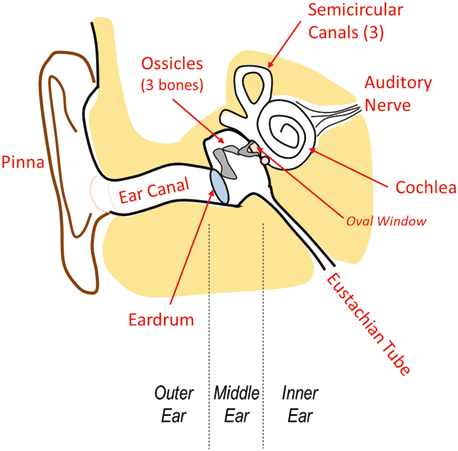
\includegraphics[height=0.9\textheight]{img/img015}
	\end{center}
\end{frame}

\subsection{Psikoakustik}

\begin{frame}
	\frametitle{Psikoakustik}
	\begin{itemize}
		\item Sebagai pendeteksi suara, sistem pendengaran manusia memiliki beberapa kekuatan dan kelemahan.
		\item Frekuensi range: 20 Hz hingga 20 kHz.
		\item Tapi kemampuan telinga dalam mendeteksi bunyi bergantung pada amplitude tekanan pada frekuensi yang diberikan, kompleksitas stimulus, dll.
		\item Investigator biasanya tidak mengutamakan fisiologi sistem pendengaran manusia saja, tapi juga persepsi bunyi.
		\item Karena beberapa kasus yang melibatkan beberapa pertanyaan terkait audibility, intelligibility, speaker identification dan testemino saksi lainnya.
	\end{itemize}
\end{frame}

\begin{frame}
	\frametitle{Kekerasan Bunyi (Loudness)}
	\begin{itemize}
		\item Tidak seperti tingkat tekanan bunyi (TTB) / sound pressure level (SPL), yang bernilai objektif. Kekerasan bunyi/ Loudness bernilai perseptual yang bergantung pada masing-masing orang.
		\item Kekerasan bunyi bergantung pada frekuensi dan juga amplitude bunyi di telinga.
	\end{itemize}
\end{frame}

\begin{frame}
	\frametitle{Equal Loudness Contours}
	\begin{center}
			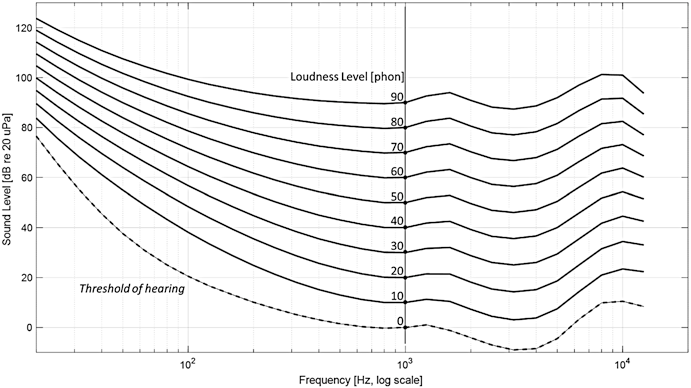
\includegraphics[width=0.9\linewidth]{img/img017}
	\end{center}
\end{frame}

\section{Referensi}

\begin{frame}
	\frametitle{Referensi}
	\begin{enumerate}
		\item Maher, R.C., (2018). Principles of Forensic Audio Analysis. New York: Springer.
		\item Auditory Brain Stem Mechanisms of Sound Localization [http://uilis.unsyiah.ac.id/oer/items/show/1217]
		%\item https://www.gaussianwaves.com/2020/01/how-to-plot-fft-in-python-fft-of-basic-signals-sine-and-cosine-waves/
	\end{enumerate}
\end{frame}

\end{document}
